\section{Saityno peržiūros sistemų architektūrų apžvalga}

\subsection{Pagrindiniai sistemos komponentai}

\subsubsection{Žvalgymo roboto „pasienis“}

\subsubsection{Parsiuntimo modulis}

\subsubsection{Saityno indekso saugyklos repozitorija}

\subsection{Sistemos UML veiklos diagrama}

\begin{figure}[ht]
\centering
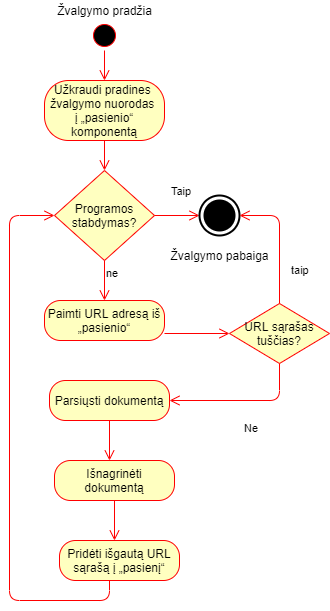
\includegraphics[scale=0.6]{img/Web_Crawler_Activity_Diagram.png}
\caption{Saityno žvalgymo roboto sistemos UML veiklos diagrama \cite{CategoriesOfWebCrawlersAndOverview}}
\label{fig:system_activity_diagram}
\end{figure}

\subsection{Viešai prieinamų sistemų realizacijų apžvalga}

Šiame skyriuje apžvelgiamos keletas žinomiausių viešuose akademiniuose literatūros šaltiniuose aprašytų saityno peržvalgos robotų sistemų architektūrų ir siekiama palyginti dizaino sprendimus įvertinant stipriąsias, silpnąsias tokių sistemų puses, rasti bendras šio tipo sistemų komponentes.

\subsubsection{„Mercator“ sistema}

1999 m. išsamiai literatūroje autorių A.Heydon ir M.Najork aprašyta ir eksperimentiškai įvertinta išplečiama, paskirstyta saityno peržvalgos roboto sistemos architektūra. Ši sistema parašyta naudojantis Java programavimo kalba ir jos vykdomąja aplinka (angl. \textit{runtime environment}). Aprašyta sistema didžiąją dalį savo aprašomų duomenų struktūrų talpina disko atmintyje, taip pat nedideli buferiai saugomi operatyvioje atmintyje ir skirti pasiekti greitesnei duomenų prieigai (kešavimo mechanizmas) \cite{MercatorLiterature}.

\subsubsubsection{Žvalgymo agentai}

Sistemoje saityno žvalgymas vyksta naudojant žvalgymo procesų gijas (angl. \textit{worker threads}, kurios veikia lygiagrečiai ir įprastai sistemoje skaičiuojamos šimtais vienetų vienu metu \cite{MercatorLiterature}. Kiekviena gija atsakinga už puslapio atsiuntimą ir apdorojimą (nuorodų suradimą, suabsoliutinimą).

\subsubsubsection{Pagrindiniai sistemos komponentai}

Aprašomos sistemos išsamesnė schema pateikiama šio rašto darbo priede. Šioje dalyje trumpai apžvelgiamos kiekvieno komponento svarbiausios charakteristikos.


\subsubsubsection{„URL siena“}

Šis komponentas (angl. \textit{URL frontier}) saugo visų lankytinų URL adresų sąrašą, sudarytas iš nepriklausomų FIFO (angl. \textit{First-In-First-Out}) principu veikiančių eilių (angl. \textit{queues}), kurių kiekviena priskiriama atitinkam žvalgymo agentui. Taip pat, kai naujas URL adresas pridedamas į kurią nors eilę, konkreti eilė apsprendžiama pagal pridedamo adreso kanoninį vardą (angl. \textit{canonical host name}). Šie du principai įgyvendina žvalgymo roboto sistemos „mandagumo“ politiką -- užtikrinama, jog daugiausiai tik vienas žvalgymo agentas apdoros konkretų saityno serverį, todėl sistema neapkraus žvalgomo serverio resursų.

\vspace{1em}
\textbf{URL adresų saugojimas}
\vspace{1em}

Kadangi saugomas URL adresų sąrašas talpina šimtus milijonų įrašų, nagrinėjamoje sistemoje jie saugomi disko atmintyje, taip pat turimas 600 adresų buferis, saugomas operatyvioje atmintyje ir leidžiantis greičiau apdoroti nuorodas (išimti, idėti).

\subsubsubsection{„HTTP protokolo modulis“}

Peržvalgos robotų sistemos turi atsižvelgti į saityno serveriuose talpinamus \textit{robots.txt} failus, įgyvendinančius REP (angl. \textit{Robots Exclusion Protocol}) ir apibrėžiančius, kokie resursai pateiktame serveryje yra leistini žvalgyti. Aprašomos sistemos HTTP modulis saugo $2^18$ eilės serverio vardo-REP failo kešą.

\subsubsubsection{Įvesties srauto komponentas}


\subsubsection{„Heritrix“ sistemos architektūra}
\subsubsection{„UbiCrawler“ sistemos architektūra}
\subsubsection{„BUbiNG“ didelio masto žvalgymo sistemos architektūra}
\subsubsection{Debesų kompiuterija grįstos sistemos architektūra}